\documentclass[./../../paper.tex]{subfiles}
\graphicspath{{\subfix{./../../figures/}}}

\begin{document}
To generate counterfactuals, we will need to establish a conceptual framework, which consists of three main components. The three components are shown in \autoref{fig:approach}. 

\attention{Change the names of the measures.}
\begin{figure}[htb]
    \centering
    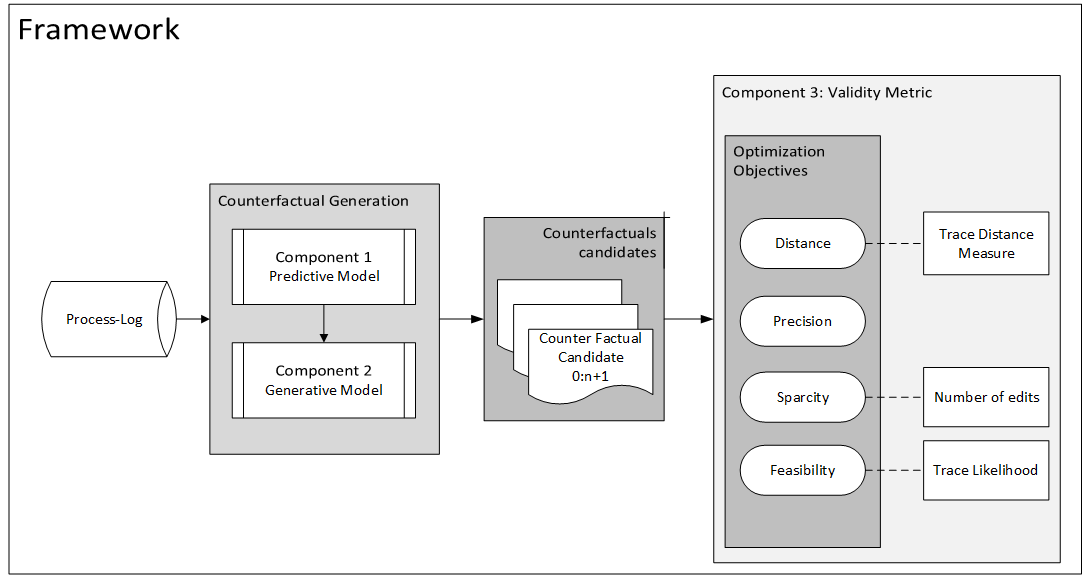
\includegraphics[width=0.99\textwidth]{figures/framework.png}
    \caption{Schows the methodoligical framework of this thesis. The input is the process log. The log will be used to train a predictive model (Component 1) and the generative model (Component 2). This process produces a set of candidates which are subject to evaluation via the validity metric (Component 3).}
    \label{fig:approach}
\end{figure}

The first component is a predictive model. As we attempt to explain model decisions with counterfactuals, the model needs to be pretrained. We can use any model that can predict the probability of a sequence. This condition holds for models trained for process outcome classification and next-activity prediction. The model used in this thesis is a simple LSTM model using the process log as an input. The model is trained to predict the next action given a sequence. 

The second component is a generative model. The generative model produces counterfactuals given a factual sequence. In our approach, each generative model should be able to generate a set of counterfactual candidates given one factual sequence. Hence, we cannot use purely deterministic generators. Therefore, we compare two different generative approaches against a baseline. The baseline uses a simple case based heuristic. The  generative approaches are a sequential a deep generative model and an evolutionary technique. Both methods allow us to use a factual sequence as starting point for the generative production but also generate multiple variations of the final solution. 

The generated candidates are subject to the third major component's scrutiny. To select the most \emph{viable} counterfactual candidate, we evaluate their viability score using a custom metric. The metric incorporates all main criterions for viable counterfactuals mentioned in \autoref{sec:counterfactuals}. We measure the \emph{similarity} between two sequences using a multivariate sequence distance metric. The \emph{precision} of the prediction will compare the likelihood of the counterfactual outcome without changes to the sequence and the counterfactual candidates. For this purpose, we require the predictive model, as it will compute the likelihoods. We measure \emph{sparcity} by counting the number of changes in the features and computing the edit distance. Lastly, we need to determine the feasibility of a counterfactual. This requires splitting the feasibility into two parts. First, the likelihood of the sequence of each event and second, the likelihood of the features given the event.



\end{document}